\documentclass[a4paper,14pt]{extreport}
  \usepackage[left=1.5cm,right=1.5cm,
      top=1.5cm,bottom=2cm,bindingoffset=0cm]{geometry}
  \usepackage{scrextend}
  \usepackage[T1,T2A]{fontenc}
  \usepackage[utf8]{inputenc}
  \usepackage[english,russian,ukrainian]{babel}
  \usepackage{tabularx}
  \linespread{1.3}
  \usepackage[colorinlistoftodos]{todonotes}
  \usepackage{amssymb}
  \usepackage{color}
  \usepackage{amsmath}
  \usepackage{mathrsfs}
  \usepackage{listings}
  \usepackage{graphicx}
  \graphicspath{ {./images/} }
  \usepackage{lipsum}
  \usepackage{xcolor}
  \usepackage{hyperref}
  \usepackage{tcolorbox}

  \usepackage[framemethod=TikZ]{mdframed}
  \usepackage{wrapfig,boxedminipage,lipsum}
  \mdfdefinestyle{MyFrame}{%
  linecolor=blue,outerlinewidth=2pt,roundcorner=20pt,innertopmargin=\baselineskip,innerbottommargin=\baselineskip,innerrightmargin=20pt,innerleftmargin=20pt,backgroundcolor=gray!50!white}
   \usepackage{csvsimple}
   \usepackage{supertabular}
  \usepackage{pdflscape}
  \usepackage{fancyvrb}
  %\usepackage{comment}
  \usepackage{array,tabularx}
  \usepackage{colortbl}

  \usepackage{varwidth}
  \tcbuselibrary{skins}
  \usepackage{fancybox}
  \usepackage{spreadtab}


  \usepackage{tikz}
  \usepackage[framemethod=TikZ]{mdframed}
  \usepackage{xcolor}
  \usetikzlibrary{calc}
  \makeatletter
  \newlength{\mylength}
  \xdef\CircleFactor{1.1}
  \setlength\mylength{\dimexpr\f@size pt}
  \newsavebox{\mybox}
  \newcommand*\circled[2][draw=blue]{\savebox\mybox{\vbox{\vphantom{WL1/}#1}}\setlength\mylength{\dimexpr\CircleFactor\dimexpr\ht\mybox+\dp\mybox\relax\relax}\tikzset{mystyle/.style={circle,#1,minimum height={\mylength}}}
  \tikz[baseline=(char.base)]
  \node[mystyle] (char) {#2};}
  \makeatother
   % Цвета для гиперссылок
  \definecolor{linkcolor}{rgb}{0, 0.72, 0.92} % цвет ссылок
  \definecolor{urlcolor}{rgb}{0.0, 0.0, 1.0}% цвет гиперссылок
  \hypersetup{pdfstartview=FitH,  linkcolor=red,urlcolor=red,citecolor=red, colorlinks=true}

  \definecolor{ggreen}{rgb}{0.4,1,0}
  \definecolor{rred}{rgb}{1,0.1,0.1}
  \definecolor{amber}{rgb}{1.0, 0.75, 0.0}
  \definecolor{babyblue}{rgb}{0.54, 0.81, 0.94}
  \definecolor{amethyst}{rgb}{0.6, 0.4, 0.8}

  \usepackage{float}
  \usepackage{wrapfig}
  \usepackage{framed}
  %for nice Code{
  \lstdefinestyle{customc}{
    belowcaptionskip=1\baselineskip,
    breaklines=true,
    frame=L,
    xleftmargin=\parindent,
    language=C,
    showstringspaces=false,
    basicstyle=\small\ttfamily,
    keywordstyle=\bfseries\color{green!40!black},
    commentstyle=\itshape\color{purple!40!black},
    identifierstyle=\color{blue},
    stringstyle=\color{orange},
  }
  \lstset{escapechar=@,style=customc}
%}


\begin{document}
\renewcommand{\bibname}{Список використаної літератури}% -- переименуем название списка литературы


%указатель -- \cite{lit1}

\pagecolor{white}

%----------------------------------------1
\newtcbox{\xmybox}[1][red]{on line, arc=7pt,colback=#1!10!white,colframe=#1!50!black, before upper={\rule[-3pt]{0pt}{10pt}},boxrule=1pt, boxsep=0pt,left=6pt,right=6pt,top=2pt,bottom=2pt}

\begin{titlepage}
  \begin{center}
  \large
  Національний технічний університет України \\ "Київський політехнічний інститут імені Ігоря Сікорського"


  Факультет Електроніки

  Кафедра мікроелектроніки
  \vfill

  \textsc{РЕФЕРАТ}\\

  %{\Large Про виконання лабораторної роботи №1\\
  з дисципліни: «Функціональна електроніка»\\[1cm]

  Функціональні пристрої на магнітостатисних спінових хвилях


  %}
  \bigskip
  \end{center}
  \vfill

  \newlength{\ML}
  \settowidth{\ML}{«\underline{\hspace{0.4cm}}» \underline{\hspace{2cm}}}
  \hfill
  \begin{minipage}{1\textwidth}
  Виконавець:\\
  Студент 4-го курсу \hspace{4cm} $\underset{\text{(підпис)}}{\underline{\hspace{0.2\textwidth}}}$  \hspace{1cm}Грабар О. О.\\
  \vspace{1cm}

  Перевірила: \hspace{5.6cm} $\underset{\text{(підпис)}}{\underline{\hspace{0.2\textwidth}}}$  \hspace{1cm}доц. Обухова Т. Ю.\\

  \end{minipage}

  \vfill

  \begin{center}
  2021
  \end{center}
\end{titlepage}
\tableofcontents
\setcounter{page}{2}

\newpage


  %\section{Подраздел}


%  \begin{figure}[h]
%   \center{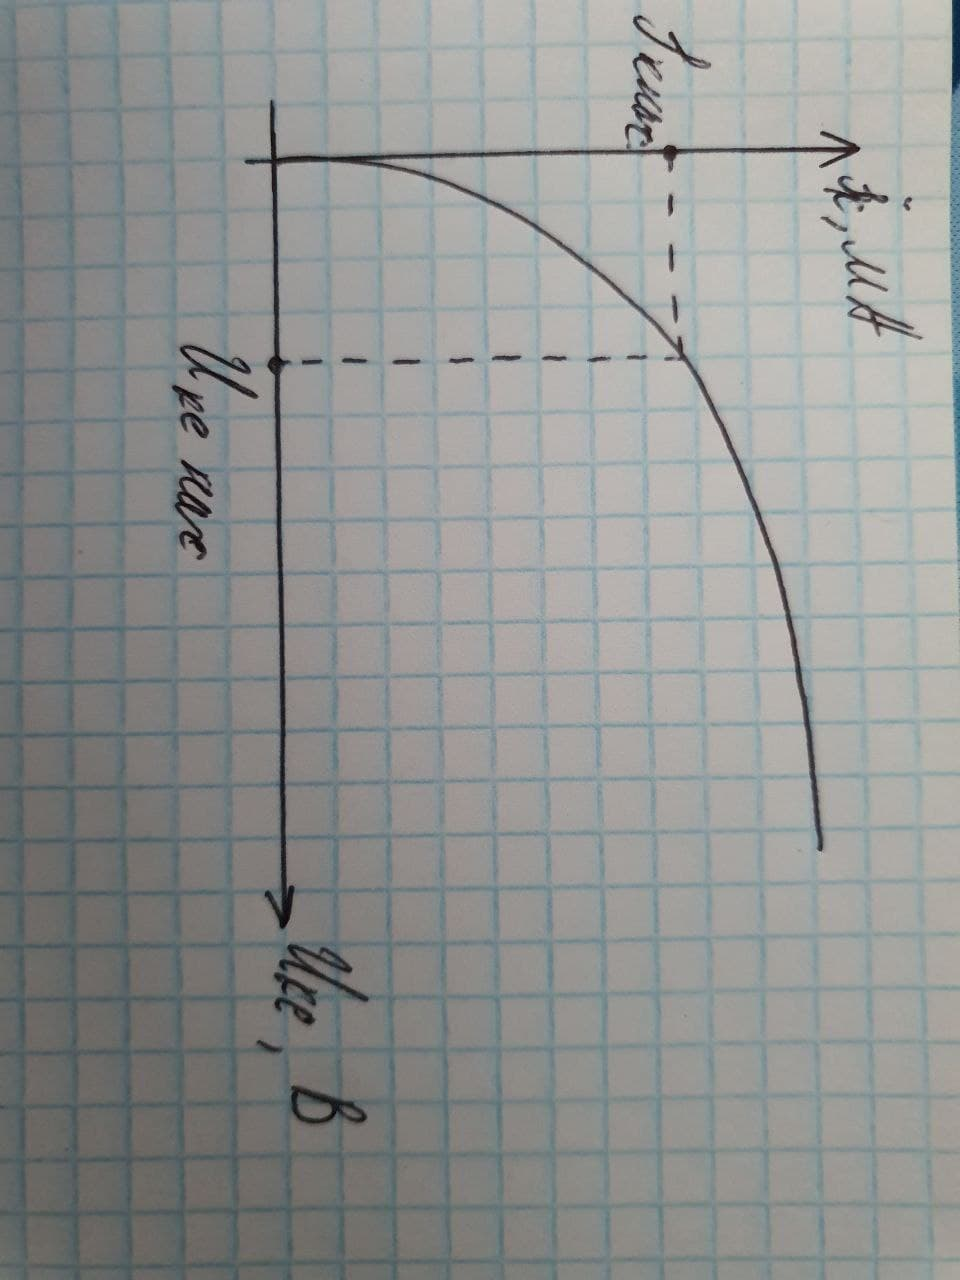
\includegraphics[width=0.9\linewidth]{2.jpg}}
%   \caption{Перший апарат магнітного запису.}
%   \label{ris2}
% \end{figure}

\chapter{ВСТУП}\par
Спін-хвильові функціональні пристрої  постійно розвиваються на основі спін-хвильових матеріалів і пов'язаних з ними ефектів. Також досягаються основні маніпуляційні процеси, необхідні для спін-хвильових логічних пристроїв, таких як зсув фази спін-хвилі, поділ сигналу і каналування. Tакож cпін-хвильові датчики  привертають все більшу увагу завдяки їх високому рівню термічної стабільності, точності. Вищезгадані розробки дозволяють спіновим хвилям знайти свою роль у сучасних  інформаційніх пристроях і не тільки. Сьогоденній прогрес  спонукає не тільки розвивати існуючу технологію
кремнієвих інтегральних схем, яка ще не вичерпала своїх можливостей, хоча все частіше
зустрічається із суттєвими труднощами та фундаментальними обмеженнями, а й проводити
дослідження і розробки альтернативних підходів, від розробки нової елементної бази
класичних обчислювальних систем на основі двійкової логіки до принципово нових підходів
в обробці інформації та сигналів: апаратних нейронних мереж, хвильових методів обчислень,
квантових обчислень\cite{lit1}, тощо.\\

Одними з таких перспективних напрямів є спін-хвильова електроніка та спінтроніка.
Основною ідеєю цих напрямів є використання спіну та колективних збуджень спінового стану
– спінових хвиль – для запису та обробки інформації. Головними перевагами цього підходу є:
(1) низькі втрати в магнітній системі порівняно з омічними втратами електричних струмів у
класичних системах, що відкриває шлях до створення елементів з наднизьким
енергоспоживанням; (2) принципова можливість суттєвої мініатюризації спін-хвильових та
спінтронних пристроїв до десятків та одиниць нанометрів; а також (3) велике різноманіття
параметричних та нелінійних ефектів у магнітних структурах, які, як, зокрема, показано в
роботі, дозволяють реалізувати не лише операції класичної двійкової логіки, а й складні
функціональні операції обробки аналогових сигналів, та застосовувати небулеві підходи до
обчислень, в тому числі, нейроморфні підходи.\\ 

Розвиток спін-хвильової електроніки розпочався у другій половині ХХ сторіччя після
відкриття та освоєння технології виготовлення монокристалів залізо-ітрієвого гранату,
магнітодіелектрика з рекордно низькими магнітними втратами, а бурхливому розвитку
спінтроніки сприяло відкриття Нобелівськими лауреатами А. Фертом та П. Грюнбергом\cite{lit1} ефекту
гігантського магнітоопору. Успішність описаного підходу підтвердило найширше
впровадження феритових пристроїв та спінтронних структур у техніку надвисоких частот та
пристрої магнітної пам’яті, відповідно.\\
 
Описане далі відноситься до нової хвилі розвитку спін-хвильової електроніки та
спінтроніки, яка розпочалась у ХХІ сторіччі і пов’язана зі стрімким розвитком технологій
виготовлення спочатку мікро-, а згодом і нанорозмірних магнітних структур. Необхідно
підкреслити, що перехід до мікро- та, особливо, наномасштабів не можна звести до простого
масштабування раніше досліджених явищ. За таких розмірів з’являються принципово нові
явища та характеристики, такі як однодоменний та односолітонний стан магнітних структур,
дискретизація спін-хвильового спектру, відбувається перехід від магнітостатичних спінових
хвиль до дипольно-обмінних та переважно обмінних спінових хвиль, радикально
підвищується роль різноманітних поверхневих та міжфазних ефектів, тощо. Хоча ці
властивості магнітних мікро- та наноструктур спричиняють труднощі, а часом накладають фундаментальні обмеження на застосування раніше розвинених підходів на малих
просторових масштабах, вони, водночас, відкривають можливості для розробки принципово
нових, часто значно ефективніших підходів до запису та обробки інформації та сигналів у
пристроях спінтроніки та спін-хвильової електроніки.\\ 




\chapter{ФУНКЦІОНАЛЬНІ СПІН-ХВИЛЬВІ ПРИСТРОЇ}\par


Пристрої обробки інформації. Спін-хвильові пристрої сприймають спін-хвилю як носій передачі та обробки інформації. У порівнянні з традиційними CMOS-пристроями, які беруть зарядний струм як носій, низьке споживання енергії є однією з найбільших переваг спін-хвильових пристроїв. Однак багато операцій наприклад, збудження, рис. 2.1(A,B) Принципова схема гетероструктури Co/GdOx та поточних електрохімічних реакцій \cite{lit3}. (A) Застосування негативної напруги зміщення викликає реакцію окислення на анод: Co буде перетворено в немагнітний матеріал CoO, і магнетизм буде усунено; (B) Застосування позитивної напруги зміщення викликає реакцію відновлення на катоді: CoO перетворюється в металевий Co, відновлюючи перпендикулярну магнітну анізотропію через Co/ Інтерфейс GdOx; (C) Зображення перехресного скануючого електронного мікроскопа накопичення водню після безперервного застосування позитивної напруги зміщення (A–C). Магніто-іонний контроль магнетизму за допомогою твердотільного протонного насоса. \\ 
\begin{figure}[h]
   \center{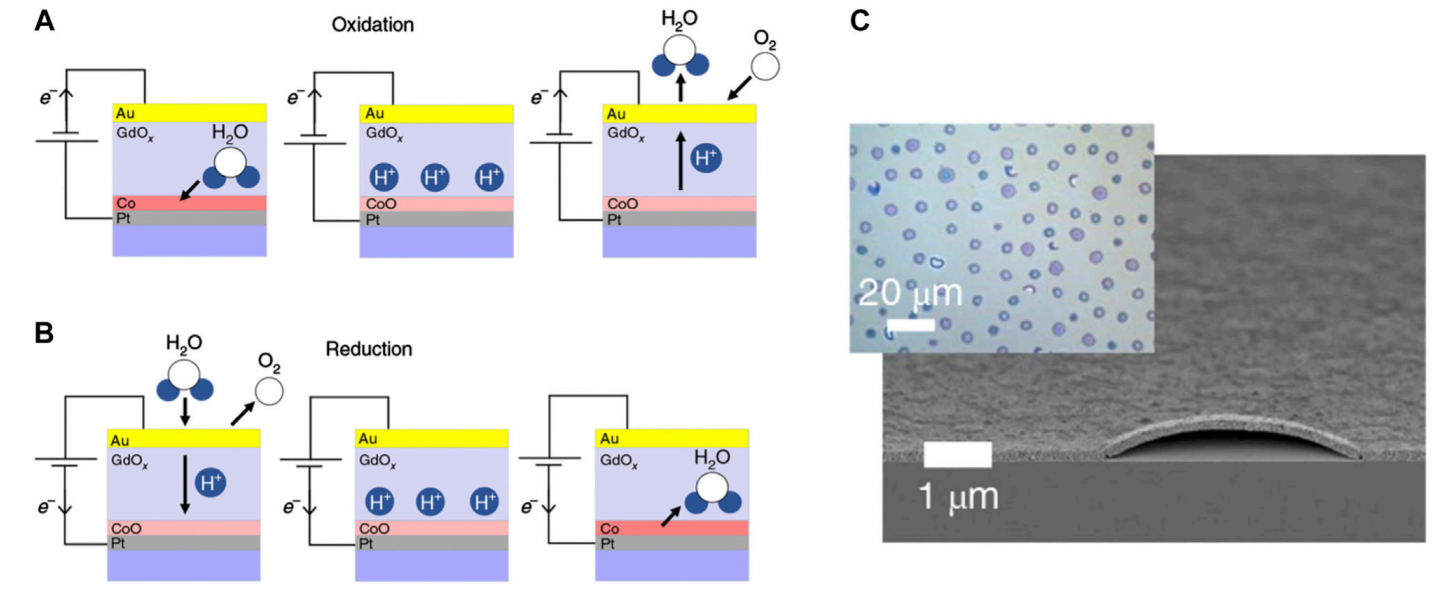
\includegraphics[width=0.9\linewidth]{5.png}}
   \caption{}
 \end{figure}

 Щоб задовольнити вимоги до наднизького енергоспоживання спін-хвильових пристроїв, недостатньо зосередитися лише на розсіювання енергії в процесі поширення спінових хвиль. Крім того, важливо зменшити розсіювання потужності під час маніпуляції зі спіновими хвилями. Це одна з головних причин постійного розвитку спін-хвильових пристроїв обробки інформації. З залученням електричного струму або напруги \cite{lit2} і різних нових ефектів інтерфейсу, дослідники розробили різноманітні спін-хвилі електронні пристрої, такі як спін-хвильовий фазовращатель, роздільник сигналу та логічний вентиль. Фазообмінник є одним з найбільш критичних компонентів спін-хвильових логічних схем. При коригуванні фаз двох або більше променів спінових хвиль з одного джерела виникає інтерференція при їх зближенні, що призводить до ослаблення або посилення сигналу спінової хвилі відповідно до логічного значення 0 або 1. \\
\begin{figure}[h]
   \center{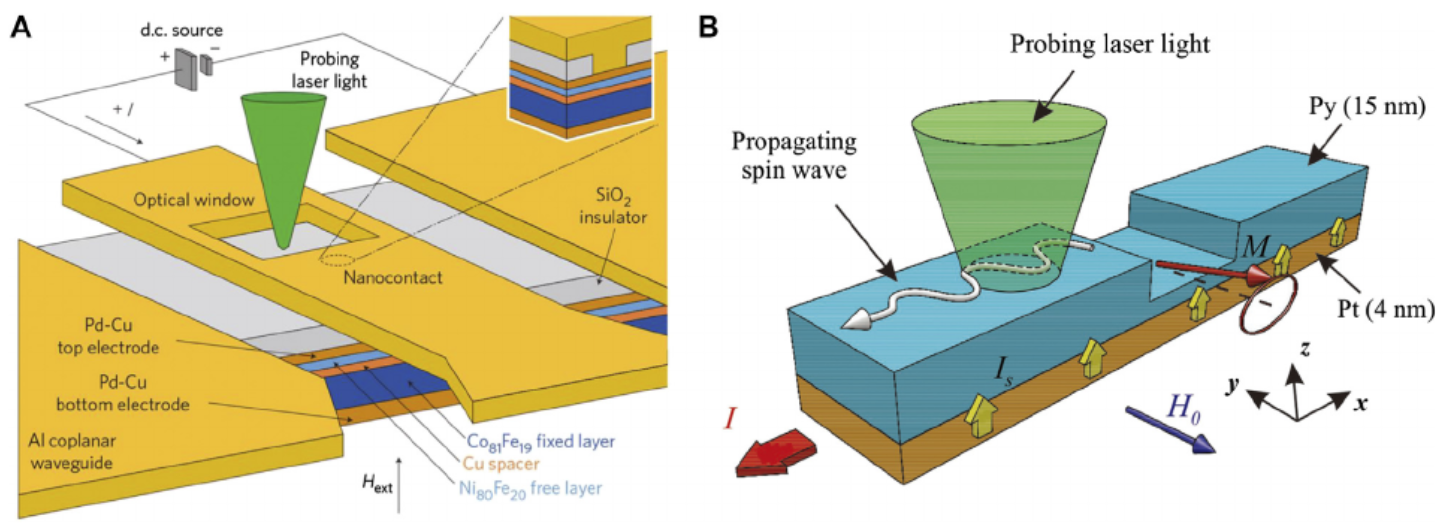
\includegraphics[width=0.9\linewidth]{6.png}}
   \caption{1}
 \end{figure}

 Електричний метод на основі струму заряду є одним з основних методів, які використовувалися в попередніх спін-хвильових електронних пристроях. У 2008 році\cite{lit6} використовували Ерстедфілд, що генерується струмом, для регулювання та проектування фазообертача, як показано на рис. 8A. Поле Ерстеда впливає на дисперсію спінової хвилі і викликає зсув фаз у спіновій хвилі. При зниженні струму поле Ерстеда зникає, і вихідні характеристики поширення спін-хвилі відновлюються. Однак у цьому методі використання електричного струму спричиняє високе споживання енергії, і відповідне джоулеве тепло може стати неприйнятним. Крім того, область застосування Ерстедфілда важко точно контролювати. Це може вплинути на інші компоненти системи. Щоб зменшити вплив джоулевого нагрівання, у 2015 році  запропонувли використовувати поляризований спіновий струм, створений ефектом STT, для безпосереднього впливу на хвилевід. Це змінило стан намагніченості початкової спінової хвилі, що призвело до фазового зсуву, як показано на рис. 8B. Результати експерименту показують, що ефект зсуву фази на 180° може бути досягнутий за допомогою трьох фазообертів. 
\begin{figure}[h]
   \center{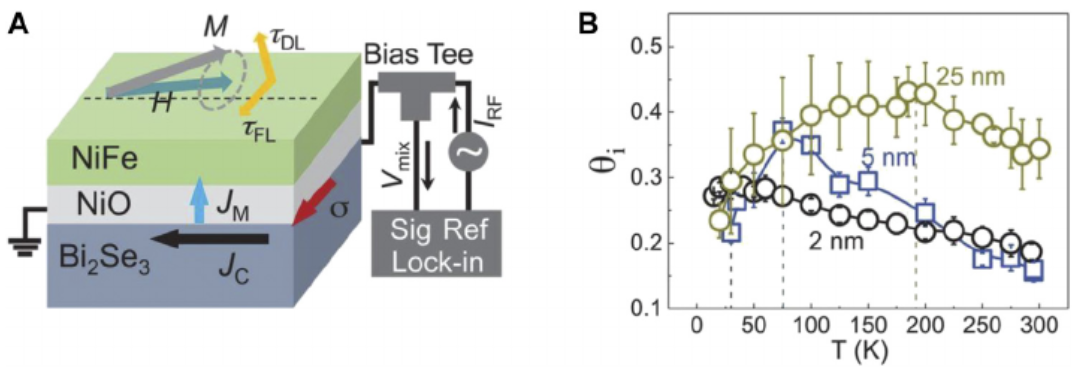
\includegraphics[width=0.9\linewidth]{7.png}}
   \caption{}
 \end{figure}

 Розділювач сигналу має велике значення для селективного перемикання спін-хвильових сигналів, де є кілька спін-хвильових каналів. У 2017 році розробили спін-хвильовий розподільник сигналу на основі зарядового струму. Як показано на рис. 8A, постійний струм прикладається вздовж осі y в коричневій області для створення поля Ерстеда, тоді як магнітне поле зміщення зовнішньої осі прикладається до всього пристрою. Спінова хвиля збуджується з лівого кінця, а потім поширюється до правого кінця. У порівнянні з вихідним випадком, в якому спінові хвилі можуть поширюватися лише під певним кутом (Рис. 2.4 B), було виявлено, що траєкторію передачі спін-хвилі можна регулювати під дією поля Ерстеда після застосування струму 100 мА (Рис. 2.4C). Це пояснюється тим, що поле Ерстеда, створене струмом, викликає відхилення в напрямку повного магнітного поля від початкового зовнішнього магнітного поля на певний кут, таким чином змінюючи дисперсію спін-хвилі і далі змінюючи траєкторію передачі. На основі цього принципу розроблений розгалужувач сигналів для з’єднання різних хвилеводів, як показано на рис. 2.4 D–F. Так як він може реалізувати перемикання та включення-вимкнення управління між різними хвилеводами, це дуже вигідно для схеми багатокаскадного каскаду. Крім того, спін-хвильовий мультиплексор був реалізований за допомогою зарядового струму, а спін-хвильовий спрямований від’єднувач був реалізований за допомогою спін-хвильового дипольного обмінного ефекту. У електронних пристроях із спін-хвильовою системою на основі зарядного струму все ще існує багато проблем. Поле Ерстеда та інші пов’язані з ним ефекти, викликані введенням струму, важко точно контролювати у всій системі. Крім того, велика кількість джоулевого тепла, що утворюється під час роботи, негативно впливає на мікро-/нано-масштабні спін-хвильові електронні пристрої. Для вирішення цієї проблеми увага досліджень була спрямована на спін-хвильові електронні пристрої, керовані напругою. У 2011 році електричне поле використовувалося для безпосереднього маніпулювання спін-хвильовою дисперсією і реалізовано ефективний контроль фази спін-хвилі під спін-орбітальним зв’язком. Як видно на рис. 2.5 А, електричне поле випромінюється від центру до кільцевого хвилеводу. Під час проходження спінової хвилі крізь хвилевід виникає низка ефектів мікрозв’язку, що призводить до фазового зсуву на 180$^\circ$. Це можна використовувати для розробки спін-хвильового інтерферометра, який потім закладає основу для розробки спін-хвильових логічних пристроїв з наднизьким енергоспоживанням. Це пояснюється тим, що процес фазового зсуву спін-хвиль не вимагає введення струму. На відміну від ефекту спін-орбітального зв’язку, інші дослідники запропонували метод конструювання спін-хвильового фазообертача, що виконується за допомогою електромагнітного зв’язку через електричне поле та взаємодії Дзялошинського-Морія (DMI). На рис. 2.5 В є принципова схема цього фазообертача. Під дією лівої області застосування електричного поля дисперсія спін-хвилі з'являється асиметричною структурою при поширенні вправо. Таким чином, різні зміщення фази виникають при різних інтенсивності електричного поля.

\begin{figure}[h]
   \center{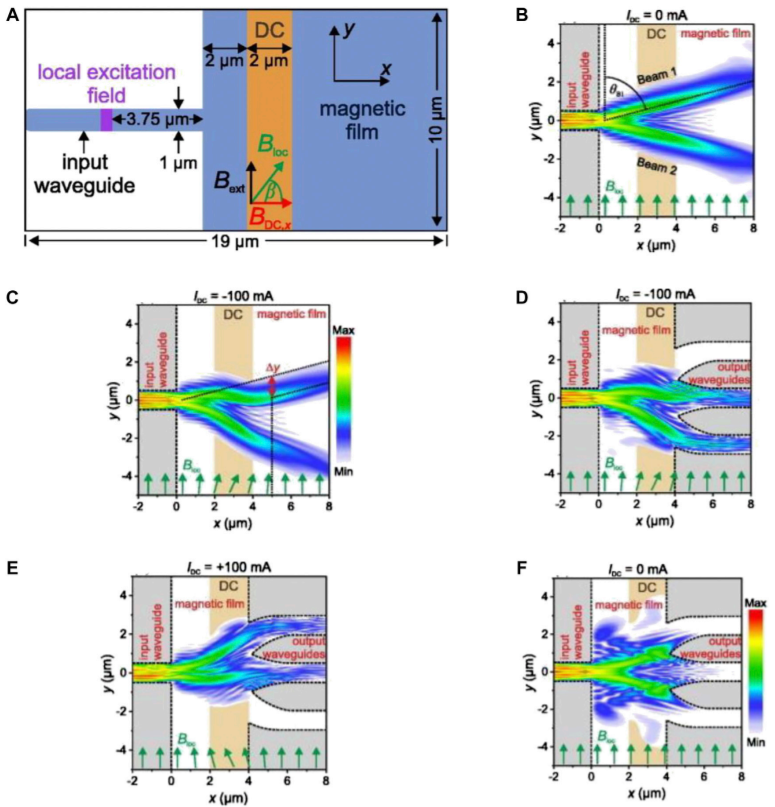
\includegraphics[width=0.9\linewidth]{8.png}}
   \caption{8}
 \end{figure}

  У магнітній анізотропії, керованої напругою, ми також обговорюємо операцію фазового зсуву спінових хвиль на основі VCMA. На додаток до електричних методів використання доменних стінок для контролю фази та амплітуди спінових хвиль є ще одним важливим методом модуляції. Рис. 2.6 A – експериментальна установка, рис. 2.6 B,C – зображення магніто-оптичного ефекту Керра (MOKE) пристроїв, на яких яскраві та темні кольори представляють домени з намагнічуванням вгору та вниз. Очевидну доменну стінку можна спостерігати в пристрої на рис. 2.6 C, тоді як пристрій на рис. 10B є однорідним. На рис. 10 D зображено змодельоване поширення спінових хвиль, верхній і нижній хвилеводи для поширення спінових хвиль, що відповідають рівномірному стану (b) і (c) стану доменної стінки відповідно. Одна пунктирна лінія вказує на вставлену доменну стінку, а пунктирна прямокутна вказує на фазовий зсув майже на 180° після проходження спінової хвилі через доменну стінку. Ханет ал. довів, що на фазовий зсув, викликаний магнітною доменною стінкою, не буде впливати конфігурація магнітного домену (тобто вгору-вниз або вниз-вгору), а відхилення п'яти експериментальних результатів фазового зсуву становить менше 10\%. Крім того, після проходження через доменну стінку амплітуда спін-хвилі зменшується в 4,3 рази.\\

\begin{figure}[h!]
   \center{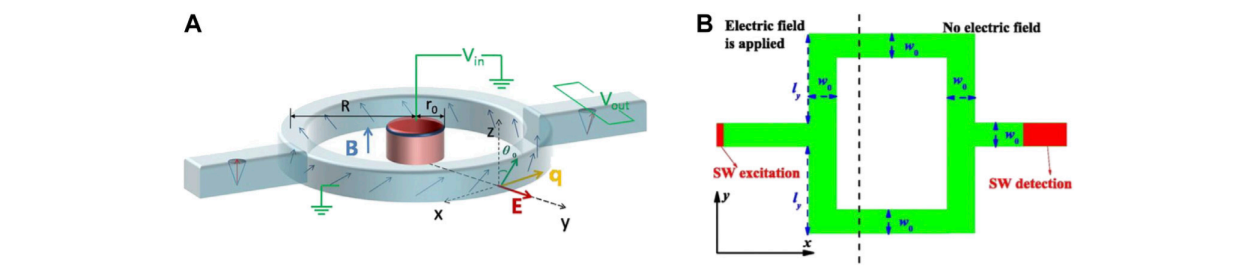
\includegraphics[width=0.9\linewidth]{9.png}}
   \caption{9}
 \end{figure}


   Це пов'язано з відображенням спінової хвилі на краю доменной стінки, викликаним квазіжорсткою граничною умовою магнітних моментів. Далі автор дослідив взаємодію між спіновими хвилями та магнітною доменною стінкою і виявив, що положення магнітної доменної стінки змінюється після проходження спінової хвилі через неї, а магнітна доменна стінка завжди рухається проти напрямку течії спінової хвилі. Це пояснюється ефектом спін-крутного моменту в магнонному струмі. Взаємний контроль між спіновими хвилями та доменною стінкою означає, що всі операції в спін-хвильових пристроях можуть бути виконані лише однією спін-хвильою.\\ 

\begin{figure}[h!]
   \center{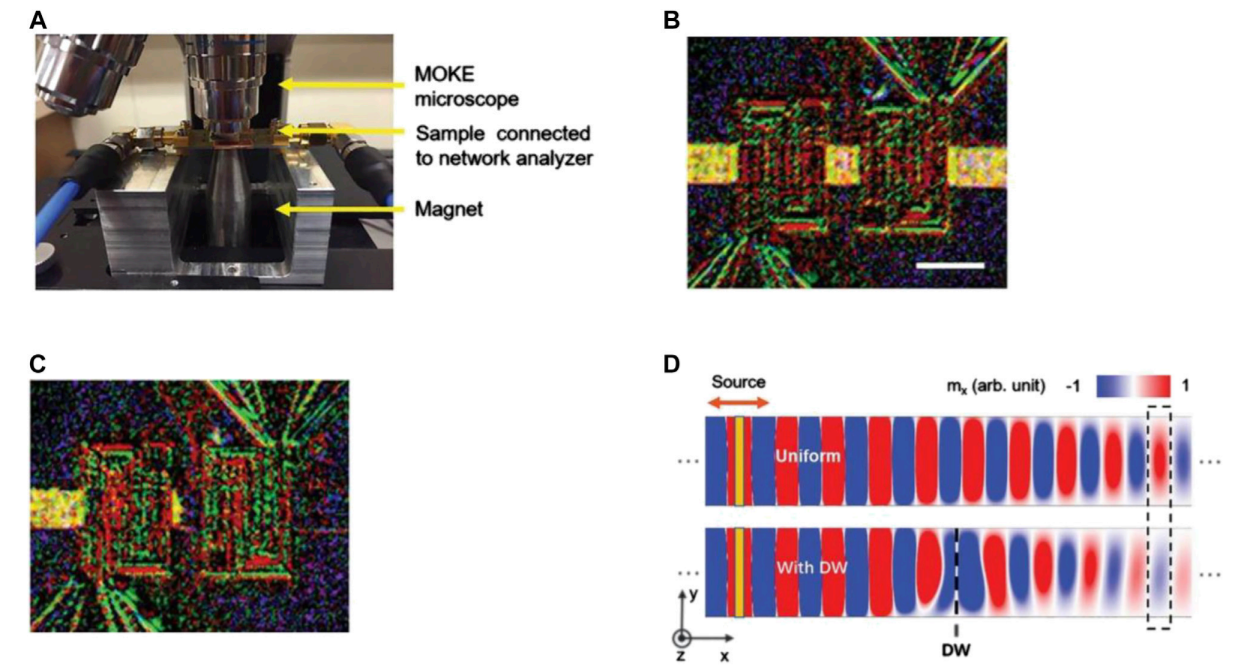
\includegraphics[width=0.9\linewidth]{10.png}}
   \caption{10}
 \end{figure}

    Це забезпечило можливість реалізації повністю магнонних спін-хвильових пристроїв. Як видно з вищенаведеного, операція фазового зсуву на основі зарядного струму пов'язана з високим рівнем споживання електроенергії, а генерується поле Ерстеда знижує точність роботи спін-хвилі. пристроїв. Розробляються нові спін-хвильові пристрої обробки інформації з низьким споживанням енергії, сумісністю з мікро-/нано-пристроями та енергонезалежністю. Кінцева мета полягає в тому, щоб реалізувати повністю керовані напругою або повністю магнонські спін-хвильові логічні пристрої, в яких спін-хвильовому пристрою, керованому напругою, потрібно лише достатньо електронів, щоб зарядити і розрядити конденсатор, а повністю магнонно-хвильовий пристрій може бути досягнутий без будь-яких втручання зовнішнього поля.

\section{Спін-хвильові датчики}\par

Датчики часто використовуються для перетворення вимірюваної інформації в інформацію, яку можна безпосередньо прочитати, наприклад, як електричні сигнали. В останні роки з безперервним розвитком досліджень магнетизму формується концепція спін-хвильових датчиків. У спін-хвильових датчиках вихід не у формі електричного сигналу, а у вигляді спін-хвильових сигналів. На додаток до ефективності енергозбереження та уникнення впливу джоулевого нагрівання є й інші причини для використання таких датчиків. Далі ми представляємо кілька спін-хвильових датчиків з різними функціями датчиків, включаючи датчики газу, магнітні датчики, і датчики вологості та далі обговорюють їхні основні принципи роботи та характеристики, спрямовані на ідентифікацію та виявлення газу, дослідники з Національного автономного університету Мексики, послідовно розроблені датчик атоксичного газу в 2015 році і покращив його продуктивність у 2017 році. Це започаткувало нову сферу досліджень «магнітних електронних носів». У цьому сенсорі магнітні наночастинки реагують з газом, щоб викликати зсув частоти до спін-хвильового осцилятора. Це забезпечує високу чутливість, короткий час відгуку, хорошу відтворюваність і можливість повторного використання. Рис. 2.7 A,B ілюструють основну структуру та принцип роботи газового датчика відповідно. Як тільки шар магнітних наночастинок вступає в реакцію з газом в навколишньому середовищі, це вплине на загальне магнітне поле сенсорної системи. Це змінює частоту коливань магнітостатичного поверхневого спін-хвильового осцилятора. Оскільки зсуви частоти, викликані різними газами, різні, датчик може ідентифікувати всі види газів. На цій основі. (2017) додали типи наночастинок і сформували масив датчиків газу, що складається з частинок $CuFe_2O_4$, $ZnFe_2O_4$, MnFe2O4 та $CoFe_2O_4$. Завдяки різній чутливості різних наночастинок до певного типу газу шляхом поєднання чотирьох результатів зондування за допомогою певних розрахунків була досягнута точність класифікації 100\%. Цей датчик газу не тільки відмінно працює, але також простий і недорогий. Однак він потребує подальших досліджень у практичних застосуваннях, таких як ідентифікація або виявлення компонентів змішаного газу та розрізнення різних газів з різними рівнями концентрацій. Датчик магнітного поля є ще одним досягненням у сфері спін-хвильових застосувань. Високоточне вимірювання магнітного поля зазвичай завершується надпровідним квантовим інтерференційним пристроєм  і гігантським магнітоімпедансним елементом. Перший вимагає наднизької температури, а якість магнітно-м’якого матеріалу, необхідного для останнього, потребує подальшого покращення. Надточний датчик магнітного поля при кімнатній температурі ще не реалізований. 

\begin{figure}[h]
   \center{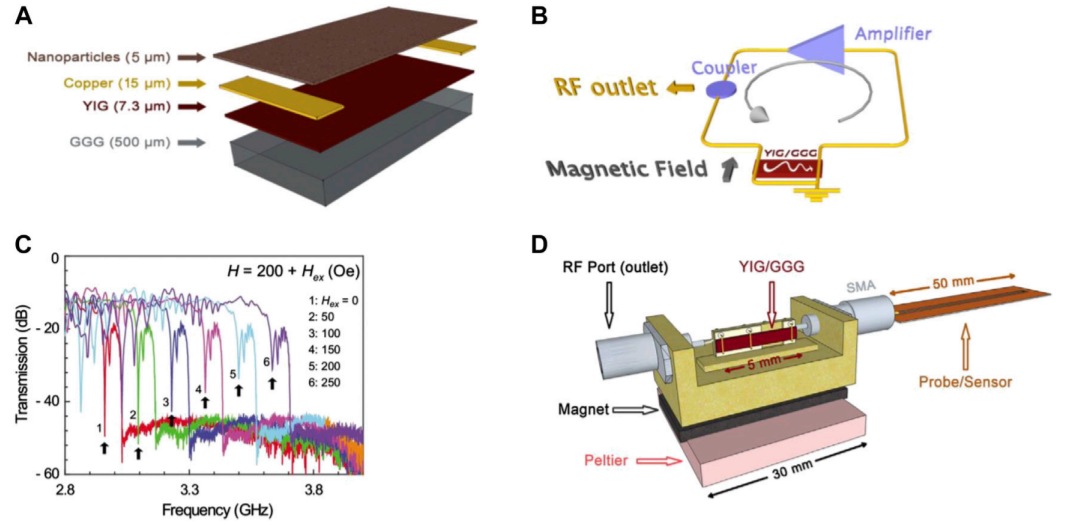
\includegraphics[width=0.9\linewidth]{11.png}}
   \caption{}
 \end{figure}



Як показано на рис. 2.7 C, чорні стрілки представляють велику зміну частоти забороненої зони зі збільшенням прикладеного магнітного поля. Зміна частоти забороненої зони впливає на характеристики поширення спін-хвилі. На основі цього принципу дослідники продемонстрували високоефективний датчик магнітного поля. Щоб вирішити проблему теплової стабільності цього датчика при високій температурі,  придушили температурну чутливість датчика за допомогою спін-хвильового диференціального каналу, що складається з двох плівок YIG. Результати показали, що термічна стабільність спін-хвильових фаз була покращена на три порядки, а точність вимірювання магнітного поля була додатково покращена. Автори показали, що запропонований ними датчик магнітного поля має чотири значущі переваги: \\ 

1) він може працювати при кімнатній температурі; \\ 

2) чутливість до поля на порядок вище, ніж у гігантського магнітоімпедансного елемента;\\ 

3) Він може вимірювати широкий діапазон магнітних полів; \\ 

4) Він має просту структуру та малий розмір. \\ 

У майбутньому датчик також може бути розроблений для вимірювання тривимірного магнітного поля (шляхом покращення розміру магнонного кристала). З постійним підвищенням точності вимірювань, очікується, що такі датчики відіграють важливу роль в інтерфейсі мозок-комп’ютер (виявлення локального тривимірного магнітного поля від мозку) та інших додатках. Вимірювання вологості є ще однією важливою функцією відчуття, яка має широке застосування в різних галузях промисловості, наприклад, зберігання продуктів харчування, високотехнологічні інструменти, фармацевтика та біомедицина. Подібно до газових Вимірювання парових сполук можна реалізувати за допомогою магнітостатичного спін-хвильового осцилятора як ключового компонента. На рис. 2.7 D показано тривимірну принципову діаграму надвисокочастотного датчика вологості. Датчик в основному складається з спін-хвильового генератора і компланарного хвилеводного зонда, в якому хвилеводний зонд вологості з'єднаний з регульованим магнітостатичним поверхневим спін-хвильовим осцилятором і поміщений у випробувальну камеру. Водопоглинаючий матеріал полівінілпіролідон (PVP) полімер покритий правокомпланарним хвилеводом. Для різних рівнів вологості відносне розширення PVP, викликане поглинанням молекул води, призводить до зміни товщини шару PVP. Потім це впливає на діелектричну проникність компланарного хвилеводного проміжку та регулює частоту коливань. Експеримент перевіряв відносну вологість у середовищі в діапазоні 12,5\%–95\%. Було виявлено, що, за винятком відносної вологості 95\%, усі інші експериментальні групи досягли понад 90\% максимального зсуву частоти протягом однієї хвилини і могли швидко відновитися до початкового стану після впливу сухого повітря. Дослідники використовують цей датчик для моніторингу дихання людини в режимі реального часу. Хоча вологість швидко змінюється внаслідок дихання, датчик здатний швидко реагувати та відновлюватися. Це дозволяє датчику швидко діагностувати респіраторні захворювання. Шляхом сполучення спін-хвилі Рис. 2.5 (A) Принципова схема.\\ 

Підводячи підсумок, принцип спін-хвильових датчиків полягає у використанні спін-хвильового осцилятора або магноного кристала для перетворення інформації в спін-хвильові сигнали (наприклад, частота спінових хвиль) для характеристики та тестування. Чи датчик газу  і датчик вологості на основі спін-хвильових осциляторів, чи датчик магнітного поля на основі магноного кристала, усі вони використовують магнітостатичну поверхневу спінову хвилю як носій вихідного сигналу. Це пояснюється тим, що spin-wavecan досягає високої частоти, а також має високе значення навантаження, низькі втрати передачі, малу довжину хвилі та високу перебудову. Ці спін-хвильові характеристики та інноваційний принцип магнетизму забезпечують набір унікальних переваг для спін-хвильових датчиків порівняно з традиційними датчиками, наприклад, більшу чутливість, меншу вартість та покращену термічну стабільність.












\chapter{ВИСНОВОК І ПЕРСПЕКТИВИ}
Було описано  ланцюжок застосування спін-хвилі в галузі
інформаційні технології. Верхній і нижній кінці ланцюга
є основними матеріалами спін-хвилі та функціональної спін-хвилі
пристроїв, відповідно. З'єднання верхнього і нижнього кінців також
досягається завдяки новим ефектам інтерфейсу. Магнітний
матеріали представлені YIG, пермаллой, CoFeB і Heusler
сплав демонструє чудові спін-хвильові властивості, укладаючи 
матеріальну основа для розвитку спін-хвилі
технології в останні кілька десятиліть, в той час як будівництво с
нова система спін-хвильових матеріалів фокусується на підготовці,
експлуатація та конструкційне проектування матеріалів. В новому
технології підготовки товщина спін-хвильових плівок
знижені при цьому їх вихідні намагнічування динамічні характеристики
підтримуються. Нові спін-хвильові матеріали використовуються в нових областях
такі як антиферомагнетики, модифікація YIG. Конструкція спін-хвильового матеріалу 
в основному знайшла своє відображення в дослідженнях магнонні кристали яких
магнітні параметри періодично змінюються.\\ 

Настроювані ефекти інтерфейсу пояснюють мікрофізичні характеристики
явища після безперервної мініатюризації спін-хвильового пристрою. VCMA є ключовим компонентом потенційного рішення
для реалізації спін-хвильових пристроїв, керованих всією напругою. Полегшений
шляхом магніто-іонного транспорту, процес управління магнетизмом
матеріалів електричним полем стає швидшим і зручнішим.\\ 

Це додатково дає можливість подальшого розвитку керованих напругою
спін-хвильові пристрої. Фізичний механізм обох ефектів STT
і ефект SOT полягає в тому, щоб швидко перевернути момент магнітного домену
за допомогою електричного обертового моменту. Цей механізм стає
дизайн ядра нової пам'яті MRAM і подальше вдосконалення
ефективність спін-хвильового збудження та посилення.
Магнон-крутний момент, відповідний електричному спін-моменту
свої особливості в плані низького споживання енергії і
велика відстань розсіювання.\\


З огляду на розвиток спін-хвильових функціональних пристроїв
проблемами є підвищення ефективності роботи пристроїв, і
зниження їх енергоспоживання. У порівнянні з
традиційні датчики, спін-хвильові датчики надають великі переваги
у вимірюванні або ідентифікації фізичних та хімічних
такі показники, як газ, магнітне поле та вологість. Ми передбачаємо
що шляхом постійного розвитку нових магнітоелектричних ефектів,
інформація про спін-хвилі з наднизьким споживанням енергії
пристрої обробки досягнуть нових кордонів у таких аспектах, як
фазовий зсув, поділ і каналування сигналу тощо.\\


З огляду на те, що закон Мура сповільнюється або навіть не працює
все ще залишається багато проблем для входу в спін-хвильовий функціонал
пристроїв на ринку, але ми можемо знайти деякі правила на майбутнє
напрямок. З точки зору спінових хвиль і спін-хвилі
матеріалів, є три аспекти, які потребують подальшого розвитку
і просування, тобто досягнення менших втрат, більш високої частоти
і стійкість поширення спінових хвиль. Існуюча спін-хвиля
матеріалом з найнижчим загасанням Гілберта є YIG, який має
досягла порядку $^{10-15}$ (мкм-товщина) шляхом рідкофазної епітаксії, але $\alpha$ матеріалів спін-хвильових сплавів, як правило, мають порядок$^{10-3}$ і потребує подальшої оптимізації (спів-хвильові сплави мають
інші унікальні переваги). Спін-хвиля охопила діапазон ГГц.
Якщо внутрішні характеристики антиферомагнітних матеріалів можуть
використовуватися, реалізація та застосування ТГц спін-хвильових пристроїв
може бути можливим при взаємодії внутрішніх сильних
обмінна зв'язок в антиферомагнетиках і зовнішня
порушення, як лазерне опромінення. Міцність віджиму
хвиля є основою передачі спінової хвилі в
складне середовище на великі відстані. Крім зменшення
магнітне загасання самого матеріалу та покращення групової швидкості спінових хвиль, можливо, ми можемо навчитися з
топологічний крайовий стан захисту в електронних топологічних ізоляторах і реалізують поширення спіну майже без втрат
хвилі на хвилеводних поверхнях, кутах або навіть дефектах.\\

З точки зору спін-хвильових функціональних пристроїв, більше
час і зусилля потрібні, перш ніж реалізувати інтеграцію, легко
регулювання та уніфіковані стандарти приладів. Немає жодних сумнівів
що інтеграція та мініатюризація пристроїв є
основний напрямок сучасного розвитку спін-хвильових пристроїв,
тому до препарату висуваються підвищені вимоги
процес (наприклад, товщина плівки, якість і простота обробки)
і надійність (наприклад, температурна стабільність) пристроїв. В
сучасні технології маніпулювання спін-хвильовими приладами
далеко не достатньо зрілі. Швидкий, простий і оборотний
необхідно знайти рішення, щоб забезпечити різноманітність і висок
ефективності функції, можливо, ми зможемо досягти мети за допомогою
прийняття методу регулювання, керованого всією напругою, на основі
динамічні магнонні кристали. Хоча нинішній хаотичний
схеми передачі спінової хвилі та стандарти для
основні матеріали повинні бути гармонізовані до спін-хвилі
інтегрований пристрій може бути успішно проданий, у нас все ще є
великі очікування щодо успіху цього процесу.












\begin{thebibliography}{9}
\bibitem{lit1} \href{http://www.kdpu-nt.gov.ua/sites/default/files/work_files/referat_signed.pdf}{: Р. В. Верба, В. О. Голуб, Г. М. Каказей, Г. А. Мелков,
О. О. Серга, О. І. Товстолиткін, А. В. Чумак, Д. Д. Шека. “Фізичні принципи спін-хвильової електроніки та спінтроніки” 2021p. }

\bibitem{lit2} <<Quantum Spin-Wave Materials, Interface Effects and Functional Devices for Information Applications>>
Jiapeng Xu, Lichuan Jin, Zhimin Liao, Qi Wang, Xiaoli Tang, Zhiyong Zhong1 and Huaiwu Zhang

\bibitem{lit3} Albisetti, E., Petti, D., Pancaldi, M., Madami, M., Tacchi, S., Curtis, J., et al. (2016).
Nanopatterning reconfigurable magnetic landscapes via thermally assisted scanning
probe lithography. Nat. Nanotechnol. 11 (6), 545.







\bibitem{lit4} Bass, J., and Pratt, W. P., Jr. (2007). Spin-diffusion lengths in metals and alloys, and
spin-flipping at metal/metal interfaces: an experimentalist’s critical review.

\bibitem{lit5} J. Phys.: Condens. Matter. 19 (18), 183201. doi:10.1088/0953-8984/19/18/183201
Bauer, U., Yao, L., Tan, A. J., Agrawal, P., Emori, S., Tuller, H. L., et al. (2015).
Magneto-ionic control of interfacial magnetism. Nat. Mater. 14 (2), 174–181.
doi:10.1038/nmat4134

\bibitem{lit6} Berger, L. (1996). Emission of spin waves by a magnetic multilayer traversed by a
current. Phys. Rev. B. 54 (13), 9353. doi:10.1103/physrevb.54.9353



\bibitem{lit7} Fulara, H., Zahedinejad, M., Khymyn, R., Awad, A., Muralidhar, S., Dvornik, M.,
et al. (2019). Spin-orbit torque–driven propagating spin waves. 

\bibitem{lit8} Gilbert, D. A., Burks, E. C., Ushakov, S. V., Abellan, P., Arslan, I., Felter, T. E., et al.
(2017). Tunable low density palladium nanowire foams. Chem. Mater.


\bibitem{lit9} Gomi, M., Furuyama, H., and Abe, M. (1991). Strong magneto-optical
enhancement in highly Ce-substituted iron garnet films prepared by
sputtering. J. Appl. Phys.

\bibitem{lit10} Gilbert, D. A., Grutter, A. J., Arenholz, E., Liu, K., Kirby, B. J., Borchers, J. A., et al.
(2016). Structural and magnetic depth profiles of magneto-ionic heterostructures 
\end{thebibliography}
\end{document}
